% Manuscript for the Journal of Trends in Computer Science and Smart Technology (IRO Journals).
% Preamble and title block follow the publisher's template
% (irojournals-scopus-paper-template-LaTex/IRO_Journals-Manuscript_LaTex_Template.tex) unchanged,
% except: amsmath and amssymb for the equations, xcolor for figure-free shading,
% and the template's "\vspace{5pt}\\" after a blank line (a LaTeX error) written without the "\\".
%
% Every number in the text comes from numbers.tex, which study/report.py generates from
% results/results.json. Build: tectonic -X compile main.tex
\documentclass[12pt,twoside]{article}
\usepackage{geometry}
\usepackage[shortlabels]{enumitem}
\setlist{nosep}
\setlist[enumerate]{wide=0pt, widest=99,leftmargin=25pt, labelsep=*}
\usepackage[none]{hyphenat}
\usepackage{graphicx}
\graphicspath{ {./} {./figures/} }
\usepackage{titlesec}
\usepackage{booktabs}
\usepackage{mathptmx}
% The template's mathptmx sets Times under pdfLaTeX. Under XeTeX (Tectonic) it sets only the maths,
% so the text gets TeX Gyre Termes, the free Times clone; pdfLaTeX builds are unchanged.
\usepackage{iftex}
\ifXeTeX
  \usepackage{fontspec}
  \setmainfont{texgyretermes}[Extension=.otf, UprightFont=*-regular, BoldFont=*-bold, ItalicFont=*-italic, BoldItalicFont=*-bolditalic]
\fi
\usepackage{setspace}
\setlength{\parindent}{0pt}
\setlength{\parskip}{1em}
\sloppy
\usepackage{array}
\newcolumntype{P}[1]{>{\centering\arraybackslash}p{#1}}
\newcolumntype{M}[1]{>{\centering\arraybackslash}m{#1}}
\newcolumntype{L}[1]{>{\raggedright\arraybackslash}p{#1}}
\titleformat{\section}
  {\normalfont\fontsize{12}{12}\bfseries}{\thesection.}{12pt}{}
\titlespacing*{\section}
  {0pt}{12pt plus 2pt minus 2pt}{0pt}
\titleformat{\subsection}
  {\normalfont\fontsize{12}{12}\bfseries}{\thesubsection}{12pt}{}
\titlespacing*{\subsection}
  {0pt}{10pt plus 2pt minus 2pt}{0pt}
\geometry{
 a4paper,
 total={170mm,257mm},
 left=2.54 cm,
 top=2.65 cm,
 right=2.54 cm,
 bottom=2.65 cm,
 }
 \rmfamily
\usepackage{fancyhdr}
\renewcommand{\footrulewidth}{0 pt}
\renewcommand{\headrulewidth}{0 pt}
\usepackage{amsmath,amssymb}

\usepackage{xcolor}
\usepackage{url}
% A visible marker for text that waits on results or author details. The submission check fails
% while any remains. review.tex defines \reviewcopy: the marker's text is then set as plain prose,
% and the author block is replaced by a note, so reviewers get a clean copy of the same sources.
\ifdefined\reviewcopy
  \newcommand{\pending}[1]{#1}
\else
  \newcommand{\pending}[1]{\textcolor{red}{\textbf{[PENDING: #1]}}}
\fi

% Generated by study/report.py from results/results.json. Do not edit by hand.
\newcommand{\nPages}{652}
\newcommand{\nChunks}{6{,}365}
\newcommand{\chunkWords}{134}
\newcommand{\nLabelled}{2{,}623}
\newcommand{\nLabelledCond}{613}
\newcommand{\nTuningPages}{40}
\newcommand{\nTuning}{209}
\newcommand{\nEval}{1{,}061}
\newcommand{\nEvalPages}{416}
\newcommand{\nEvalCond}{560}
\newcommand{\nEvalUncond}{400}
\newcommand{\nEvalUnans}{101}
\newcommand{\nEvalOpposite}{88}
\newcommand{\nRamQ}{500}
\newcommand{\nRamMulti}{400}
\newcommand{\nRamMisinfo}{243}
\newcommand{\sepCond}{72.1}
\newcommand{\sepUncond}{42.2}
\newcommand{\condOnly}{38.7}
\newcommand{\condApart}{14.0}
\newcommand{\goldChunksCond}{2.18}
\newcommand{\goldChunksUncond}{1.59}
\newcommand{\sepCondHundred}{82.9}
\newcommand{\sepCondThreeHundred}{46.3}
\newcommand{\sepCondSection}{68.5}
\newcommand{\recAnsEight}{74.0}
\newcommand{\recCondEight}{74.5}
\newcommand{\recCondOnlyEight}{67.7}
\newcommand{\recAllGoldEight}{58.9}
\newcommand{\recLostGivenAnsEight}{8.0}
\newcommand{\recUncondAnsEight}{79.3}


\begin{document}

 \begin{singlespace}
 \begin{center}
\fontsize{24}{24}\selectfont\textbf
{Where Do the Conditions Go? Stage-wise Attribution of Condition Loss in Chunked Retrieval-Augmented Generation}
\end{center}
\vspace{24pt}
\ifdefined\reviewcopy
\begin{center}\fontsize{11}{11}\selectfont\textit{Revised manuscript, review copy. Author names, affiliations and biographies are omitted.}\end{center}
\else
\fontsize{16}{16}\selectfont\textbf{
Author Name$^1$, Author Name$^2$}
\vspace{16pt}\\
\fontsize{11}{11}\selectfont {
$^1$Department, College, University, City, Country \\
$^2$Department, College, University, City, Country
}\vspace{16pt}\\
{\fontsize{9}{9}\selectfont\textbf{{E-mail:}} $^1$author1@college.edu, $^2$author2@institute.com}\\
\fi

\end{singlespace}
\fontsize{12}{12}\selectfont
\begin{onehalfspace}
\section*{Abstract}
Retrieval-augmented generation (RAG) is increasingly used to answer questions from official guidance, where an answer often holds only under a condition. We ask where, in a chunked RAG pipeline, such conditions are lost. On ConditionalQA, turned into open retrieval over all \nPages{} of its gov.uk pages, the benchmark's human annotation lets us measure chunking, retrieval and evidence-reducing operators directly, and generation with the official metric under one shared prompt; an analysis plan fixed before any evaluation run defines the tests. Chunking separates the conditions of \sepCond\% of conditional questions from their answers, and losing the chunks that hold only a condition costs two local generators about five points of F1 with conditions. Retrieval is not biased against conditions, and the distractors it retrieves dilute the context more than its misses do. A reranker, a contradiction filter and a ConflictRAG-style resolver delete condition chunks as readily as answer chunks, yet change end-to-end scores little, because generation is the dominant loss: with every condition in context, even a 550B-parameter model leaves two thirds of them unstated. On RAMDocs, where discarding is correct, the same operators fail to isolate misinformation. A trained qualifier-aware context completion does not help, and its scorer does not transfer. We release all code, splits and model outputs.

\par\vspace{5pt}\noindent
\textbf{\fontsize{12}{12}\selectfont Keywords:} retrieval-augmented generation; conditional question answering; chunking; evidence selection; knowledge conflicts; evaluation

\section{{Introduction}}

Much of what people ask about public services has an answer that holds only under a condition. Can I bring my other child on this visa? Yes, if that child also has or is applying for a Child Student visa. Do I have to keep payroll records? Yes, for at least six years, if they were created after a certain date. An answer stripped of its condition is not merely incomplete; for the person whose situation does not meet the condition, it is wrong, and it is stated with the confidence of a correct one.

Retrieval-augmented generation (RAG) \cite{lewis2020rag} is now a common way to answer such questions from official guidance. A RAG pipeline never reads a guidance page whole. It reads \emph{chunks}: pieces of fixed size cut from each page, retrieved by similarity to the question, often filtered or reranked, and then passed to a language model. Each of these steps can separate an answer from the condition that limits it, and each can do so silently, since the answer that remains is fluent and partly right.

At the same time, a large body of work makes RAG pipelines more selective about evidence, because retrieved passages can be irrelevant or false \cite{xu2024survey}. Relevance graders drop passages judged unhelpful \cite{yan2024crag}; conflict resolvers detect contradicting passages and keep the more credible one \cite{conflictrag2026}; consolidation methods keep what they judge reliable \cite{wang2025astute}. These modules are designed and evaluated where removing evidence is the right thing to do, such as misinformation. They are rarely evaluated where the passage that looks least relevant, or most contradictory, is an exception to the rule beside it.

This paper asks a measurement question: \emph{where, in a chunked RAG pipeline, are the conditions of an answer lost?} We answer it on ConditionalQA \cite{sun2022conditionalqa}, whose answers are annotated by people with the conditions under which they hold, turned into an open-retrieval task over all \nPages{} of its gov.uk pages. Because the human annotation identifies every condition as an exact element of its page, the first three stages of the pipeline can be measured directly, with no language model in the loop: whether chunking separates a condition from its answer, whether retrieval finds it, and whether an evidence-reducing module keeps it. The fourth, generation, is measured with the benchmark's official metric, under a single generator prompt shared by every system so that systems differ only in the evidence they pass on.

Our main findings are as follows.
\begin{enumerate}[(1)]
\item \textbf{Chunking separates conditions from answers.} With 150-word chunks, the gold evidence of \sepCond\% of conditional questions spans more than one chunk, against \sepUncond\% of unconditional ones; for \condOnly\% of conditional questions some condition sits in a chunk that holds nothing else the answer needs.
\item \textbf{Retrieval is not biased against conditions, except those chunked apart.} Condition chunks are retrieved as often as answer chunks (\recCondEight\% and \recAnsEight\% at $k=8$), but chunks that hold only a condition are retrieved less (\recCondOnlyEight\%).
\item \textbf{Evidence-reducing operators are blind to conditions.} A reranker, a contradiction filter and a ConflictRAG-style resolver remove retrieved condition chunks at the same rate as answer chunks; the contradiction filter fires on \nliChanged\% of questions about a single, consistent body of guidance, because an exception reads as a contradiction of its rule. On RAMDocs \cite{wang2025madam}, where discarding is the point, the same operators do not single out misinformation either.
\item \textbf{Generation is where most conditions are lost.} With every condition in context, the two local generators state \recallGoldQwen\% and \recallGoldLlama\% of the gold conditions as conditions on their answer, and the largest of three larger hosted models \hRecallNemo\%; the official metric, meanwhile, rewards a generator for rarely stating conditions at all.
\end{enumerate}

End to end, two local generators and three larger hosted ones agree on the order of these losses (Sections~\ref{sec:endtoend} and~\ref{sec:hosted}). Losing an isolated condition chunk from otherwise complete evidence costs every generator measurably; retrieval at an equal budget costs about a point; the operators, despite their deletions, change little for small generators, which have already lost most conditions in generation; and the larger generators, which state more conditions, lose more at every stage before generation. We also test a remedy aimed at the retrieval side, \emph{qualifier-aware context completion}, which adds the same-page chunks that a cross-fitted scorer predicts state a condition. It helps none of the five generators, and its scorer neither beats an untrained reranker nor transfers to a separately annotated corpus. We report it as a negative result: the lever is the generator, not the context.

The contributions of this paper are: (i) a stage-wise, annotation-grounded measurement of condition loss in chunked RAG; (ii) the first evaluation of evidence-reducing and conflict-handling operators on ConditionalQA, contrasted with the same operators on RAMDocs; (iii) a pre-registered test of qualifier-aware context completion, a cross-fitted remedy trained only on the benchmark's existing annotation, which does not help; and (iv) all code, the fixed question splits, every model output and an analysis plan committed before the first evaluation run.

\section{Related Work}

\subsection{Conflicting evidence and evidence-reducing RAG}

Retrieval-augmented generation conditions a language model on passages retrieved for the query \cite{lewis2020rag}. Because retrieved passages can be irrelevant, outdated or wrong, much work adds modules that decide which passages to trust; Xu et al.\ \cite{xu2024survey} survey conflicts between contexts and between context and the model's memory. Corrective RAG \cite{yan2024crag} grades each retrieved document and acts on the grade; Astute RAG \cite{wang2025astute} consolidates internal and external knowledge by source reliability; MADAM-RAG \cite{wang2025madam} has one agent per document debate, and introduces RAMDocs, which mixes ambiguity, misinformation and noise. ConflictRAG \cite{conflictrag2026} types each detected conflict and resolves factual ones by Entropy-TOPSIS credibility selection, temporal ones by recency and opinion conflicts by presenting several perspectives.

Two recent results are close in spirit to ours. CONFLICTS \cite{cattan2025conflicts} argues that the right behaviour depends on the conflict type, and specifies a different desired response for each. Ragability \cite{gross2026ragability} finds that warning a model of contradictions helps it detect them but hurts when there are none. Kumar \cite{kumar2026verification} shows that gating chunks one by one with an entailment check is worse than not filtering on multi-hop questions, since a chunk that does not entail the answer alone can still be necessary. We study a third case in which reducing evidence can hurt: the passage a module removes or never retrieves is the one that states \emph{when} the answer holds.

\subsection{Conditional answers}

ConditionalQA \cite{sun2022conditionalqa} annotates every answer with the conditions under which it holds, on UK government guidance; human performance on conditional answers with their conditions is much lower than on the rest of the benchmark. Chain of Condition \cite{lin2024chaincondition} prompts a language model to identify the conditions in a document, build their logical relations, and verify and resolve them against the scenario; evaluated mainly with gold passages, it improves how a reader handles the conditions it is given, not whether the pipeline gives them. Our study is complementary: it holds the reader fixed and measures where conditions are lost; our verification pass (Section~\ref{sec:diagnostics}) is a simple instance of Chain of Condition's identify-and-verify step. Defeasible scope has also been studied within single legal provisions: Chen et al.\ \cite{chen2026sgdt} parse statutes into span-grounded deontic trees and name the failure of dropping a defeater \emph{silent scope omission}. Their setting keeps a rule and its exceptions in one provision; ours asks what happens when chunking puts them in different passages.

\subsection{Chunking and retrieval granularity}

What a retriever indexes changes what it finds: Dense~X \cite{chen2024densex} shows that the retrieval unit (passage, sentence or proposition) affects both retrieval and downstream answers, and DAPR \cite{wang2024dapr} builds a benchmark of passages that need their document's context to be retrieved, ConditionalQA among them, on which adding the document title to each passage helps. Work on legal texts reports that fixed-size chunking separates basic rules from their exceptions \cite{prior2026chunking}, but does not measure how often or with what consequence. Closest to our setting, Wan et al.\ \cite{wan2026retrieverfree} retrieve from all ConditionalQA guides split into paragraphs and report retrieval hit rates and answer exact match; conditions are not evaluated.

\subsection{Multi-hop evidence, sufficiency and defeasible inference}

A condition chunked apart from its answer resembles a missing hop in multi-hop retrieval, since two passages are needed together, but the resemblance is partial. In multi-hop questions the second passage is needed to reach the answer at all, so losing it shows up as a wrong answer; a condition qualifies an answer that can be reached without it, so losing it shows up only as missing scope, which answer-centric metrics do not register. Per-chunk gating removes necessary bridge passages on multi-hop benchmarks \cite{kumar2026verification}; we measure the analogous removal for conditions, whose cost answer accuracy does not show. Joren et al.\ \cite{joren2025sufficient} classify whether a retrieved context suffices for a definitive answer, and find that models often answer rather than abstain when it does not; a context that has lost a condition can still support a definitive answer, so it is insufficient in a sense such a check does not test. In the terms of defeasible reasoning \cite{chen2026sgdt}, ConditionalQA's conditions are defeaters written into the source; we ask whether a pipeline delivers them and whether the generator states them.

\textbf{Our position.} Table~1 sets the closest lines of work against this study. We found no prior work that measures against human annotation how often an answer's conditions are lost in chunked open retrieval, attributes the loss to its stages, or evaluates conflict-handling operators where discarding is and is not correct; the novelty claim is limited to this combination, not to any one of its parts.

\begin{table}[!htbp]\centering
\textbf{Table 1.} The closest lines of work and what this study adds.\\\vspace{5pt}
{\fontsize{9}{11}\selectfont
\begin{tabular}{L{2.5cm}L{2.85cm}L{4.4cm}L{4.4cm}}
\toprule
\textbf{Line of work} & \textbf{Representative work} & \textbf{What it measures} & \textbf{What this study adds} \\
\midrule
Conflict handling and evidence reduction & CRAG \cite{yan2024crag}, Astute RAG \cite{wang2025astute}, ConflictRAG \cite{conflictrag2026}, MADAM-RAG \cite{wang2025madam}, CONFLICTS \cite{cattan2025conflicts}, Ragability \cite{gross2026ragability} & whether modules remove irrelevant, false or conflicting passages, or respond to the type of conflict & the same evidence-reducing steps where a removed passage can be a valid condition, with deletion rates measured against human annotation \\
Multi-hop evidence and sufficiency & Kumar \cite{kumar2026verification}, Joren et al.\ \cite{joren2025sufficient} & whether bridge passages survive filtering; whether a context suffices to answer & the loss of passages that qualify an answer reachable without them, which answer accuracy does not register \\
Conditional answers & ConditionalQA \cite{sun2022conditionalqa}, Chain of Condition \cite{lin2024chaincondition}, Wan et al.\ \cite{wan2026retrieverfree} & readers' answers and conditions given gold passages; open retrieval scored without conditions & conditions scored under chunked open retrieval, stage by stage, with the reader held fixed \\
Defeasible and scoped rules & Chen et al.\ \cite{chen2026sgdt} & rules and their defeaters parsed within one legal provision; silent omission of a defeater & defeaters that chunking separates from the rule they qualify \\
Chunking and retrieval granularity & Dense X \cite{chen2024densex}, DAPR \cite{wang2024dapr}, Prior et al.\ \cite{prior2026chunking} & how the retrieval unit and document context affect retrieval; rule--exception splitting, described qualitatively & how often conditions are separated and at what cost, with context-preserving retrieval designs compared (Section~\ref{sec:retrieval}) \\
\bottomrule
\end{tabular}
}
\end{table}

\section{{Methodology and Experimental Design}}
\label{sec:method}

\subsection{Applicability conditions and how a pipeline can lose them}

A question about a policy often has an answer that holds only under a condition the asker has not settled. A person asks whether they can bring another child on a Parent of a Child Student visa; the guidance says yes, \emph{if} the child also has or is applying for a Child Student visa. Neither ``yes'' nor ``no'' is a correct answer on its own: the correct answer is ``yes, provided that \dots''. We call the clause that must also hold an \emph{applicability condition}.

Formally, a question $q$ with scenario $s$ has a gold answer set $A(q)=\{(a_i, C_i)\}$, where $a_i$ is an answer and $C_i$ is the set of condition statements under which $a_i$ holds and which $s$ leaves unresolved. A question is \emph{conditional} when some $C_i \neq \emptyset$. The statements in $C_i$, together with the statements that give $a_i$ itself (its \emph{answer evidence} $E_i$), are passages of a source document $d(q)$.

A retrieval-augmented pipeline never sees $d(q)$ whole. It sees chunks. Let $\kappa$ be a chunking function that partitions a document into chunks, and let $\kappa(x)$ denote the chunk holding statement $x$. For each conditional question we define
\begin{equation}
\mathrm{Sep}(q) = \mathbf{1}\Big[\big|\{\kappa(x) : x \in \textstyle\bigcup_i (C_i \cup E_i)\}\big| > 1\Big],
\end{equation}
the event that the gold no longer fits in one chunk, and the set of \emph{condition-only chunks}
\begin{equation}
\mathcal{K}_C(q) = \{\kappa(x) : x \in \textstyle\bigcup_i C_i\} \setminus \{\kappa(x) : x \in \textstyle\bigcup_i E_i\},
\end{equation}
chunks that carry a condition and nothing else the answer needs. A chunk in $\mathcal{K}_C(q)$ is exactly the kind of passage a pipeline can drop while still producing a fluent, confident and partly correct answer.

Applicability conditions take several logical forms: eligibility requirements (``if you are over 18''), exceptions (``unless the ATF repairs the vehicle''), time limits, prohibitions and conditional permissions. ConditionalQA's annotators mark as a condition any statement an answer depends on that the scenario leaves open, whatever its form, and we follow their annotation rather than impose a finer taxonomy; the forms are not distinguished in any result below. Conditional evaluation questions carry \annMeanCond{} condition elements on average, \annTwoPlus\% have two or more, and \annMultiAnswer\% have more than one answer, each with its own conditions.

A condition can be lost at four stages, which this work separates:
\begin{enumerate}[(i)]
\item \textbf{Chunking} places it in a chunk apart from the answer.
\item \textbf{Retrieval} ranks that chunk below the cut-off $k$.
\item \textbf{Evidence reduction}: a reranker, relevance grader, contradiction filter or conflict resolver removes the chunk after retrieval.
\item \textbf{Generation}: the condition is in the context and the model does not state it, or states a condition that does not apply.
\end{enumerate}

\subsection{Testbed: ConditionalQA as chunked open retrieval}

ConditionalQA v1.0 \cite{sun2022conditionalqa} is built on \nPages{} UK government guidance pages from gov.uk; every answer is annotated with the conditions under which it holds, and every condition and evidence statement is quoted verbatim as an HTML element of its page (a paragraph, list item, table row or heading). We turn it into open retrieval over the whole collection.

\textbf{Chunking.} Each page is cut into chunks of whole elements, packed greedily up to 150 words, so the chunk holding every gold statement is known exactly and $\mathrm{Sep}(q)$ and $\mathcal{K}_C(q)$ follow directly from the annotation: \nChunks{} chunks, mean \chunkWords{} words, each prefixed for retrieval with its page title and nearest section heading.

\textbf{Questions.} The test answers are not public, so we evaluate on the labelled training and development questions; all systems are zero-shot, so both are unseen to them. Before running any system we fixed a document-disjoint split: every question on \nTuningPages{} random pages forms a \emph{tuning} set (\nTuning{} questions), the only place prompts and thresholds were chosen; the \emph{evaluation} set holds every conditional (\nEvalCond{}) and unanswerable (\nEvalUnans{}) question on the other pages and \nEvalUncond{} random unconditional ones, \nEval{} questions on \nEvalPages{} pages.

\textbf{Retrieval.} BM25 \cite{robertson2009bm25} and Contriever \cite{izacard2022contriever} rankings are fused by reciprocal rank \cite{cormack2009rrf} over all chunks; the query is the question followed by the scenario, and the rankings are shared by every system.

\subsection{One generator, many evidence policies}

Every system is defined by one thing, \emph{which chunks reach the generator}; the generator, its instructions and its output format are identical for all, so any difference between two systems is a difference in their evidence. The generator sees the chunks as numbered lines, one per HTML element, with the scenario and question, and returns JSON listing each answer with the lines that state it (\emph{evidence}) and the lines that state a requirement which must also hold and which the scenario does not settle (\emph{conditions}); condition lines are mapped back to their exact elements, the form the official metric scores. Four worked examples from the tuning pages precede the question. Separating evidence from conditions was the one change the tuning set showed to matter (Section~\ref{sec:generation}). Because citations are line numbers, a condition cannot be missed through paraphrase: a gold condition in context is cited as a condition, cited as evidence, or not cited.

\textbf{Generation settings.} Decoding is greedy (temperature 0). Lines are numbered in page order, identically for every model, and each model receives the same messages through its provider's chat template. The output budget is 768 tokens for the local models, 3{,}072 for gpt-oss-20b (low reasoning effort) and 1{,}024 for Gemma-4-31B and Nemotron-3-Ultra; the local context window is 8{,}192 tokens; at most five answers are scored. An output that is not valid JSON in the required shape, is cut off at the token limit, or is aborted by the server as a repetition loop counts as unanswered; provider errors are retried, and the recorded answer is the model's first complete output. Prompts, examples and settings are in the repository.

Table~1 lists the systems, in three families. \textbf{The oracle ladder} isolates stages by construction: \texttt{gold\,$-$\,cond.\ elements} measures how much the metric depends on conditions being present at all; \texttt{gold\,$-$\,cond.-only chunks} is what a pipeline delivers when it finds the answer and loses a separately chunked condition; \texttt{gold\,+\,distractors} gives perfect recall under realistic distraction; a closed-book run measures what the models answer from memory. \textbf{Evidence-reducing operators} start from the top 8 and reproduce modules common in robust RAG stacks: a cross-encoder reranker (checkpoint \texttt{BAAI/bge-reranker-base}, BGE family \cite{xiao2024cpack}); a contradiction filter built on an NLI cross-encoder \cite{he2023debertav3} (an NLI judgement says only that two passages cannot both hold as stated, not which is authoritative or whether one qualifies the other, which is precisely the case at issue); a ConflictRAG-style resolver \cite{conflictrag2026}; relevance grading in the manner of corrective RAG \cite{yan2024crag}; and listwise selection, a single-call reduction of Astute RAG's consolidation \cite{wang2025astute}. The resolver is a partial reproduction, since the authors' code is not released: it scores three of the original five credibility criteria (source authority, recency and specificity), omitting the relevance and consistency criteria the original extracts with a language model, and on gov.uk pages authority and recency tie, so specificity decides; our results concern this implementation, not the published system. \textbf{Context completion}, described next, adds chunks instead; its budget-matched baselines add chunks without any knowledge of conditions.

\begin{table}[!htbp]\centering
\textbf{Table 2.} The systems. Each differs only in which chunks reach the same generator. Operators are marked by how closely they follow the method they are named after: [S] a standard component, not a reproduction; [P] a partial reproduction; [R] a reduction of the method to its evidence-reducing step. $^\dagger$\,Exploratory in the analysis plan; $^\ddagger$\,added in revision (exploratory, except the clean threshold protocol, a corrected re-analysis that is primary for completion).\\\vspace{5pt}
{\fontsize{9}{11}\selectfont
\begin{tabular}{L{4.3cm}L{10.6cm}}
\toprule
\textbf{System} & \textbf{Chunks given to the generator} \\
\midrule
\multicolumn{2}{l}{\emph{Oracle ladder (uses the gold annotation; not deployable)}}\\
\texttt{closed-book} & none \\
\texttt{gold} & exactly the chunks holding the annotated evidence and conditions \\
\texttt{gold\,$-$\,cond.\ elements} & the same chunks with the condition elements deleted \\
\texttt{gold\,$-$\,cond.-only chunks} & the gold chunks minus those holding only conditions \\
\texttt{gold\,+\,distractors} & all gold chunks, filled to 8 with top-ranked non-gold chunks \\
\midrule
\multicolumn{2}{l}{\emph{Retrieval}}\\
\texttt{top-$k$} & the $k$ highest-ranked chunks, $k\in\{3,8\}$ (recall alone is measured up to $k=50$); \texttt{top-8} is the reference \\
\midrule
\multicolumn{2}{l}{\emph{Evidence-reducing operators (applied to the top 8)}}\\
\texttt{rerank-3} & [S] the 3 chunks a cross-encoder reranker scores highest \\
\texttt{NLI filter} & [S] drops the lower-ranked chunk of each pair judged contradictory \\
\texttt{ConflictRAG-style} & [P] resolves each detected conflict by Entropy-TOPSIS credibility selection (3 of 5 criteria) \\
\texttt{relevance grading}$^\dagger$ & [R] corrective RAG's grading: keeps the chunks the generator model grades as useful, one call each (RAMDocs only) \\
\texttt{listwise selection}$^\dagger$ & [R] Astute RAG's consolidation in one call: keeps the chunks the generator model selects \\
\midrule
\multicolumn{2}{l}{\emph{Context completion (budget of 8 chunks)}}\\
\texttt{adjacent}$^\dagger$ & the top 5 plus the chunks next to them on their pages \\
\texttt{page}$^\dagger$ & every chunk of the top-ranked chunk's page \\
\texttt{completion (untrained)}$^\dagger$ & the top 5 plus same-page chunks scored by an off-the-shelf reranker \\
\texttt{completion} (ours)$^\ddagger$ & the top 5 plus same-page chunks a trained scorer predicts state a condition; each fold's scorer and threshold set without any evaluation label \\
\texttt{completion (pre-reg.\ $\tau$)} & the same, with the pre-registered threshold, chosen under a scorer trained on the evaluation folds \\
\midrule
\multicolumn{2}{l}{\emph{Context-preserving retrieval$^\ddagger$ (budget: the words of the top 8)}}\\
\texttt{sentence window} & single elements retrieved, each passed with two neighbours on either side \\
\texttt{parent-child} & single elements retrieved, each passed with its top-level section \\
\texttt{hierarchical} & the top 2 pages retrieved first, then their 8 highest-ranked chunks \\
\texttt{query expansion} & the top 8 chunks for the query extended with condition cue words \\
\bottomrule
\end{tabular}
}
\end{table}


\subsection{Qualifier-aware context completion}

We test one remedy aimed at the retrieval side, stated as a hypothesis: if the retriever has reached the right page but not the chunk that qualifies the answer, a scorer trained on the benchmark's condition annotation can find that chunk among its neighbours. By design it can only add chunks from pages the top chunks already reached; Section~\ref{sec:completion} measures how often the missing condition lies there. Qualifier-aware completion keeps the top $k_0=5$ retrieved chunks and adds, from the pages those chunks come from, the chunks most likely to state a condition on the answer, up to the same budget of eight chunks as \texttt{top-8}.

For a question $q$ with scenario $s$, let $P$ be the (at most two) pages of the top-$k_0$ chunks and, for each page $p\in P$, let $a_p$ be its highest-ranked retrieved chunk, the \emph{anchor}. Every other chunk $c$ on $p$ that was not retrieved is a candidate, scored by a cross-encoder $f_\theta$:
\begin{equation}
\sigma(c) = f_\theta\big([\,q;\, s;\, a_p\,],\; c\big) \in [0,1].
\end{equation}
The system adds the candidates with $\sigma(c)\geq\tau$, highest first, up to $8-k_0$ of them, and leaves the remaining slots empty: it adds qualifiers, not context for its own sake.

$f_\theta$ is DeBERTa-v3-base \cite{he2023debertav3} fine-tuned to predict whether a candidate chunk holds a gold condition element of the question. The labels are ConditionalQA's own annotation, so no new labelling is needed; unconditional questions contribute negatives only, which is what teaches the scorer when to add nothing. To keep every question scored by a model that never saw its page, training is \emph{cross-fitted}: the evaluation questions are split into five document-disjoint folds, and the model that scores a fold is trained on the other four folds and the tuning set. The tuning questions are scored by a model trained on all five evaluation folds, and $\tau$ is chosen on them alone. That model has seen evaluation labels, but it never scores an evaluation question; it only sets $\tau$, and Section~\ref{sec:completion} shows that no threshold, even one chosen on the evaluation questions themselves, makes the scorer accurate, so the choice of $\tau$ cannot account for the result. A second variant, \texttt{completion (untrained)}, scores candidates with the off-the-shelf reranker on $(q, c)$ instead, to separate what training contributes from what any relevance model would give. A third, \texttt{completion (oracle)}, added in revision, adds exactly the candidates that hold a gold condition: it shows what the architecture could gain with a perfect scorer.

\subsection{A secondary diagnostic: the contrast regime}

ConditionalQA is the primary evaluation. RAMDocs \cite{wang2025madam} serves only as a secondary diagnostic, and its limits come first: its misinformation is synthetic, \nRamMulti{} of its \nRamQ{} questions have several valid answers for same-name entities, so it mixes ambiguity with conflict, and it has no training split. Its absolute scores are therefore not comparable with ConditionalQA's, and we draw from it only one contrast. Removing evidence is not always wrong: when some retrieved passages are false, discarding them is the purpose of the operators above. Because each RAMDocs document is labelled correct, misinformation or noise, it allows an \emph{oracle discard} system that removes exactly the misinformation and noise, the ceiling for any operator that removes evidence, and so asks whether the same operators that cannot tell a condition from a contradiction can at least tell a false document from a true one. A RAMDocs answer is correct when it contains every gold answer and no wrong answer.

\subsection{Metrics and inference}

The primary metric is ConditionalQA's official \emph{F1 with conditions}, computed by the authors' evaluation script, unchanged. For one gold answer $(a, C)$ and one predicted answer $(\hat a, \hat C)$ it is
\begin{equation}
\mathrm{F1}_c = \mathrm{F1}_{\mathrm{tok}}(\hat a, a)\cdot
\begin{cases}
\mathbf{1}[\hat C=\emptyset] & \text{if } C=\emptyset,\\
\mathrm{F1}_{\mathrm{set}}(\hat C, C) & \text{otherwise,}
\end{cases}
\end{equation}
where $\mathrm{F1}_{\mathrm{tok}}$ is SQuAD token F1 and $\mathrm{F1}_{\mathrm{set}}$ is the F1 of exact element matches. Over several answers the script takes the best one-to-one assignment and multiplies by $\exp(1-|\hat A|/|A|)$ when more answers are predicted than exist. The metric therefore cannot be raised by verbosity: listing extra answers is discounted, and naming a condition where the gold has none scores zero. Because this score rewards a generator that never states a condition on unconditional questions, we never read it alone. We also report answer F1 (conditions ignored), the precision and recall of predicted condition elements, exact match with conditions (answer and conditions both exactly right), the share of unconditional answers that name any condition (false conditions), how the gold conditions in context are handled by the generator (stated as conditions, cited only as evidence, or not cited), and, for unanswerable questions, the share left unanswered.

Questions on the same page share chunks and retrieval behaviour, so they are not independent. Every interval and test treats the \emph{page} as the unit: differences between two systems are paired by question, with 95\% BCa bootstrap intervals over pages (2{,}000 resamples) and page-level sign-flip permutation tests (20{,}000 permutations). The confirmatory comparisons, listed in the analysis plan we committed before the first evaluation run, are corrected by the Holm procedure \cite{holm1979} separately for each model.

\textbf{Models.} The two primary generators run locally on a consumer GPU: Qwen2.5-7B-Instruct \cite{qwen2024qwen25} and Llama-3.1-8B-Instruct \cite{grattafiori2024llama3}, both 4-bit quantised, at temperature 0. To test whether the direction of the main effects holds at larger scale, we repeat the key systems on a stratified subsample of \nHostedQ{} evaluation questions with three larger open-weight models from three families: gpt-oss-20b \cite{openai2025gptoss}, a mixture of experts served by Groq and, once Groq's daily quota is spent, by NVIDIA's API with identical settings (Section~\ref{sec:hosted} checks the two providers against each other on the same questions); Gemma-4-31B (NVIDIA API identifier \texttt{google/gemma-4-31b-it}; the checkpoint published as \texttt{google/gemma-4-31B-it}), a dense model; and Nemotron-3-Ultra (\texttt{nvidia/nemotron-3-ultra-550b-a55b}), a hybrid mixture of experts with 55B of its 550B parameters active, run with its reasoning mode off, both served by NVIDIA. Every answer records the provider that served it. These are reported as replication, not as confirmatory tests. The models differ in architecture, training, quantisation and serving as well as in size, so their comparison is not a controlled scaling experiment. Qwen3.8-27B (Groq model identifier \texttt{qwen/qwen3.8-27b}) was used only in prompt tuning (Section~\ref{sec:generation}).

\textbf{Diagnostics added in revision.} Four exploratory analyses were added after the confirmatory results, and are recorded as such in the analysis plan. (i) A \emph{condition-verification pass}: after the frozen generator has answered, a second call to the same model receives the same lines, the scenario, the question and the answers, and lists for each answer the lines that state a requirement the scenario does not settle; the answers are kept and only their conditions replaced. It tests whether a dedicated check recovers the conditions the generator ignores. (ii) \texttt{completion (oracle)}, described above. (iii) The \texttt{top-8} and \texttt{gold} systems with section-aware chunks instead of 150-word chunks, end to end, with a fixed 70-word chunking whose mean size matches the section-aware chunks as a control. (iv) Every gpt-oss-20b gold-context question that Groq served is asked again on NVIDIA's API.

\textbf{Transfer corpus.} The out-of-distribution check of the completion scorer uses a corpus from the authors' earlier work: \nOodCorpus{} query-and-passage-pair instances from gov.uk immigration guidance and UK bank terms, labelled for conflict type and scope relation (a refinement is a pair in which one passage states a rule and the other a condition or exception to it), including written probe pairs and distractor pairs with no conflict. Each instance carries two annotators' labels, but no valid inter-annotator agreement was established for it, so its labels are treated as provisional and the check as indicative only.

\section{{Results and Discussion}}

We follow a condition through the pipeline in order; the first three stages are measured against the human annotation without any language model, the fourth with the official metric.

\subsection{Chunking separates conditions from the answers they qualify}
\label{sec:chunking}

With 150-word chunks, the gold of \sepCond\% of conditional questions no longer fits in a single chunk, against \sepUncond\% of unconditional ones; a conditional question needs \goldChunksCond{} gold chunks on average against \goldChunksUncond. For \condOnly\% of conditional questions at least one condition sits in a chunk holding no other evidence the answer needs. Larger chunks reduce separation without removing it: \sepCondThreeHundred\% are still split at 300 words (mean \chunkWordsThreeHundred{} words) and \sepCondHundred\% at 100 (mean \chunkWordsHundred). Structure, not size, is what helps: section-aware chunks (a new chunk at every top-level heading, mean \chunkWordsSection{} words) split \sepCondSection\% and isolate a condition in \condOnlySection\% of conditional questions, while size-matched fixed 70-word chunks split \sepCondSeventy\% and isolate one in \condOnlySeventy\%. On gov.uk pages conditions are typically list items under a lead-in sentence or paragraphs below a rule, so the structure that states a condition is the structure a word budget cuts.

\subsection{Retrieval finds conditions as often as answers, except those chunked apart}
\label{sec:retrieval}

At $k=8$ the hybrid retriever returns \recAnsEight\% of answer chunks and \recCondEight\% of condition chunks of conditional questions, and the two curves stay together at every depth (Figure~2). The exception is the chunk that holds a condition and nothing else: only \recCondOnlyEight\% are retrieved at $k=8$, and they trail the other curves until $k=50$. The full gold reaches the generator for \recAllGoldEight\% of conditional questions, and when every answer chunk has been retrieved a condition chunk is still missing in \recLostGivenAnsEight\% of cases: the configuration that yields a confident answer without its caveat. Section-aware chunks cover less text at the same $k$, so condition recall falls to \recCondEightSection\% and complete-gold recall to \recAllGoldEightSection\%.

\textbf{Context-preserving retrieval designs do not consistently improve condition coverage.} Held to the top 8's word budget (\blWordsTop{} words on average), sentence windows, parent--child sections, hierarchical page-then-chunk retrieval and condition-expanded queries give a condition coverage (the share of gold condition elements of conditional questions in the context) of \blRecallSentwin\%, \blRecallParent\%, \blRecallHier\% and \blRecallQexp\%, against \blRecallTop\% for the top 8, and the whole gold for \blCompleteSentwin\%, \blCompleteParent\%, \blCompleteHier\% and \blCompleteQexp\% of questions, against \blCompleteTop\%. End to end, on the answerable questions of the hosted subsample, the four designs change F1 with conditions on conditional questions against the top 8 by \blCondMin{} to \blCondMax{} points across the two local generators; \blCondNSig{} of these \blNRuns{} differences, and \blUncondNSig{} on unconditional questions, are distinguishable from zero.

\begin{figure}[!htbp]\centering
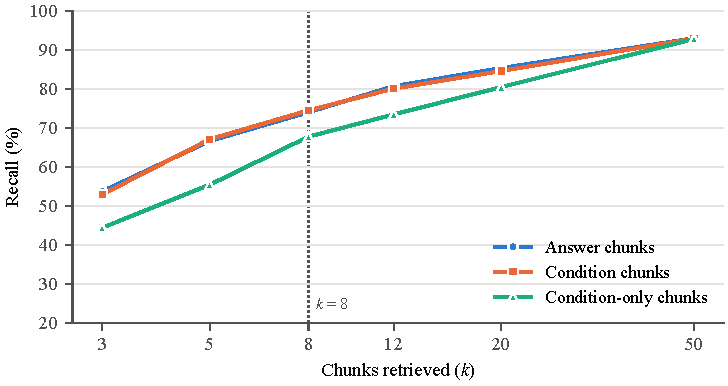
\includegraphics[width=0.56\textwidth]{recall.pdf}
\vspace{3pt}\\
\textbf{Figure 2.} Recall of gold chunks against retrieval depth for the \nEvalCond{} conditional evaluation questions (hybrid retrieval over \nChunks{} chunks). Condition-only chunks hold a condition and no other gold evidence.
\end{figure}

\subsection{The evaluated operators do not distinguish conditions}
\label{sec:operators}

The model-free operators choose chunks before any answer is generated, so their effect on conditions is measured directly (Figure~3, left). Reranking the top 8 down to 3 removes \rrCondDrop\% of the retrieved condition chunks and \rrAnsDrop\% of the answer chunks. The contradiction filter changes the context of \nliChanged\% of conditional questions, although every passage comes from one consistent body of guidance, and removes \nliCondDrop\% of condition chunks and \nliAnsDrop\% of answer chunks; the ConflictRAG-style resolver changes \crsChanged\% of contexts and removes \crsCondDrop\% and \crsAnsDrop\%. None of them targets conditions, and none protects them. To an NLI model an exception contradicts the rule it qualifies: for one evaluation question the filter kept ``You'll get a `Certificate of Destruction' to prove that the vehicle has been destroyed'' and dropped, with contradiction probability 1.00, the gold condition ``You will not get a certificate of destruction if the ATF decides to repair and sell your vehicle''. On RAMDocs, where removing documents is the purpose, the same operators do not single out misinformation either (Figure~3, right): reranking keeps \ramRrMisinfo\% of misinformation documents and \ramRrCorrect\% of correct ones, since a document with one entity swapped is exactly as relevant as the original, and the filter keeps \ramNliMisinfo\% and \ramNliCorrect\%.

\begin{figure}[!htbp]\centering
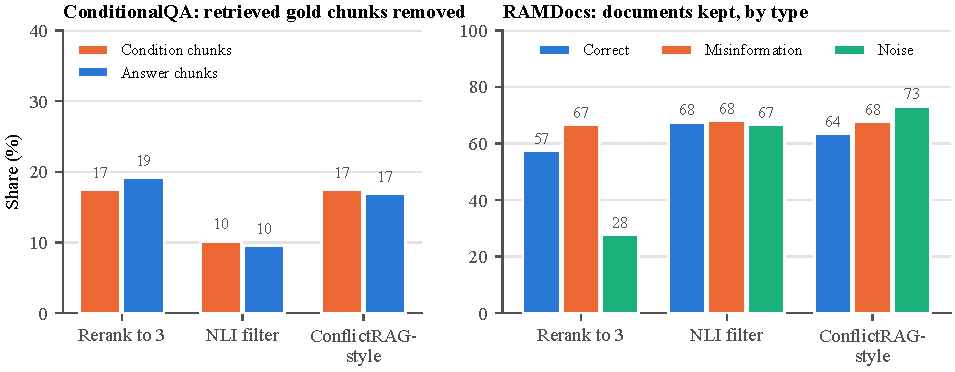
\includegraphics[width=0.78\textwidth]{operators.pdf}
\vspace{3pt}\\
\textbf{Figure 3.} Left: share of the gold condition and answer chunks retrieved in the top 8 that each operator removes (\nOpCond{} conditional evaluation questions with a retrieved condition chunk). Right: share of RAMDocs documents each operator keeps, by type (\nRamQ{} questions).
\end{figure}

\subsection{Generation and the choice of prompt}
\label{sec:generation}

Already on the tuning set, with exactly the gold chunks in context, the generators mark only \tunRecallQwen\% (Qwen2.5-7B), \tunRecallLlama\% (Llama-3.1-8B) and \tunRecallBig\% (Qwen3.8-27B) of the gold conditions as conditions, and F1 with conditions on these questions is \tunFcCondQwen, \tunFcCondLlama{} and \tunFcCondBig{}, against 56.6 for the benchmark's human annotators \cite{sun2022conditionalqa}. The metric rewards silence: a stated condition scores zero whenever the gold has none, as for most questions. For Qwen2.5-7B, a wording that discourages conditions (v2) cut the unconditional answers naming one to \tunAnyCondUncondVTwo\% and raised F1 with conditions on unconditional questions to \tunFcUncondVTwo, while it fell to \tunFcCondVTwo{} on conditional ones. We froze the wording that states the benchmark's own definition of a condition (v4: \tunFcCondQwen{} and \tunFcUncondVFour), not the one with the best overall score, because a generator that rarely states conditions cannot lose one, and every comparison of evidence policies would then show no effect by construction.

Is the generation deficit then a property of this prompt? Table~3 answers the hosted subsample with the gold chunks under five condition-aware strategies besides the frozen one (analysis v). No strategy removes the deficit. Across six prompts and three generators, the share of gold conditions stated as conditions ranges from \prMinRecall\% to \prMaxRecall\%, and is at most \prMaxRecallLocal\% for the local models. Against the frozen prompt, \prNSigGain{} of the \prNRuns{} variant runs raise F1 with conditions on conditional questions by an amount distinguishable from zero (largest change \prMaxGain{} points) and \prNSigLoss{} lower it; the largest gain, answer--condition pairing with Nemotron-3-Ultra, still states only \prRecallNemoPairing\% of the gold conditions and changes F1 with conditions on unconditional questions by \prVsUncondNemoPairing. The strategies that state more conditions attach them to more unconditional answers too: direct extraction raises the condition recall of Llama-3.1-8B from \prRecallLlamaVFour\% to \prRecallLlamaExtract\% and of Nemotron-3-Ultra from \prRecallNemoVFour\% to \prRecallNemoExtract\%, but changes F1 with conditions on unconditional questions by \prVsUncondLlamaExtract{} and \prVsUncondNemoExtract, and \prNSigLossUncond{} of the \prNRuns{} variant runs are significantly worse there. Chain-of-condition reasoning, whose identify-and-verify steps target exactly this failure, gives condition recall of \prRecallQwenCoc\%, \prRecallLlamaCoc\% and \prRecallNemoCoc\%, against \prRecallQwenVFour\%, \prRecallLlamaVFour\% and \prRecallNemoVFour\% with the frozen prompt. Removing the condition-only chunks lowers F1 with conditions under \prCTwoPos{} of the \prCTwoN{} prompt--generator combinations, so the chunking cost does not depend on the prompt either. The deficit is not an artefact of one wording, though it remains a finding about the strategies we evaluated.

% Generated by study/report.py. Do not edit by hand.
\begin{table}[!htbp]\centering
\textbf{Table 3.} The generation deficit under six prompts, with the gold chunks in context (hosted subsample: 150 conditional, 100 unconditional questions). Rec.: share of gold conditions stated as conditions (\%); on U: share of unconditional answers that name any condition (\%); F1c: F1 with conditions on conditional / unconditional questions (\%). The first row is the frozen prompt; the other five were added in revision (exploratory) and share its lines, worked examples and output format.\\\vspace{5pt}
{\fontsize{9}{11}\selectfont
\setlength{\tabcolsep}{3.5pt}
\begin{tabular}{L{3.3cm}P{0.8cm}P{0.8cm}P{1.75cm}P{0.8cm}P{0.8cm}P{1.75cm}P{0.8cm}P{0.8cm}P{1.75cm}}
\toprule
 & \multicolumn{3}{c}{\textbf{Qwen2.5-7B}} & \multicolumn{3}{c}{\textbf{Llama-3.1-8B}} & \multicolumn{3}{c}{\textbf{Nemotron-3-Ultra}} \\
\textbf{Prompting strategy} & Rec. & on U & F1c C / U & Rec. & on U & F1c C / U & Rec. & on U & F1c C / U \\
\midrule
frozen: the benchmark's definition & 21.6 & 36.0 & 10.0 / 30.7 & 18.1 & 26.0 & 15.2 / 59.2 & 32.1 & 17.0 & 19.2 / 58.3 \\
direct condition extraction & 15.1 & 46.0 & 11.2 / 21.0 & 28.2 & 45.0 & 16.0 / 42.1 & 42.5 & 38.0 & 19.6 / 47.1 \\
answer--condition pairing & 23.8 & 36.0 & 13.2 / 33.9 & 16.4 & 25.0 & 13.6 / 50.2 & 38.6 & 22.0 & 24.5 / 53.6 \\
chain-of-condition reasoning & 11.2 & 22.0 & 5.1 / 26.8 & 20.8 & 47.0 & 11.3 / 36.0 & 30.7 & 15.0 & 18.4 / 58.3 \\
applicability check per line & 15.6 & 28.0 & 10.4 / 32.8 & 11.2 & 28.0 & 9.1 / 55.6 & 36.7 & 25.0 & 18.9 / 54.4 \\
evidence first, roles labelled & 14.8 & 39.0 & 7.7 / 18.4 & 20.0 & 46.0 & 12.9 / 38.2 & 35.9 & 28.0 & 19.7 / 48.2 \\
\bottomrule
\end{tabular}
}
\end{table}


\subsection{End to end: where the conditions are lost}
\label{sec:endtoend}

Table~4 lists every system on the evaluation set and Table~5 the pre-registered tests; the two local generators agree on every confirmatory comparison but the last. \textbf{The metric measures condition use:} deleting the condition elements from the gold chunks lowers F1 with conditions by \cOneQwenPt{} for Qwen2.5-7B and \cOneLlamaPt{} for Llama-3.1-8B (C1). \textbf{Chunking costs conditions:} on the \nCondOnlyEval{} conditional questions with a condition-only gold chunk, removing those chunks from the gold context costs \cTwoQwenPt{} and \cTwoLlamaPt{} (C2), although everything else the answer needs is present. \textbf{Retrieval costs a little; dilution costs more:} at an equal budget of eight chunks, the gold chunks filled up with distractors beat the top 8 by \cThreeQwenPt{} and \cThreeLlamaPt{} (C3), so most of the distance between the gold chunks and the top 8 (\fcGoldQwen{} against \fcTopQwen{} for Qwen2.5-7B, \fcGoldLlama{} against \fcTopLlama{} for Llama-3.1-8B) is what retrieval adds, not what it misses.

\textbf{The operators change nothing measurable at this scale.} Reranking, the contradiction filter and the ConflictRAG-style resolver each leave F1 with conditions within about a point of the top 8 (C4--C6), although they remove \rrCondDrop\%, \nliCondDrop\% and \crsCondDrop\% of the retrieved condition chunks: these generators state so few conditions that there is little to lose, citing \noticedTopQwen\% and \noticedTopLlama\% of the condition lines they are shown in the top 8. \textbf{Context completion does not help:} under the clean threshold protocol it changes F1 with conditions against the top 8 by \clCSevenQwenPt{} and \clCSevenLlamaPt{} (C7; Holm-adjusted $p$ of \clCSevenHolmQwen{} and \clCSevenHolmLlama), and on unconditional questions it meets the non-inferiority margin of 2 points for Qwen2.5-7B (lower bound \clCEightLowQwen) but not for Llama-3.1-8B (\clCEightLowLlama); the pre-registered protocol gives \cSevenQwenPt{} and \cSevenLlamaPt{} (C7$^{\mathrm{p}}$) and the same non-inferiority verdicts. Of the exploratory policies only listwise selection, in which the reader itself chooses the chunks, gains for both generators (\eSevenQwen{} and \eSevenLlama), distinguishably from zero only for Llama-3.1-8B. \textbf{Closed-book answering is a sobering baseline:} without evidence, Qwen2.5-7B scores \fcClosedUncondQwen{} on unconditional questions, far above the \fcTopUncondQwen{} it reaches with the top 8, which tempts it to attach a condition to \anyCondTopUncondQwen\% of answers that need none. On the \nOppositeQwen{} conditional questions whose gold contains both ``yes'' and ``no'', the gold chunks beat the top 8 by \eSixQwen{} and \eSixLlama{}, the same direction as on all conditional questions.

% Generated by study/report.py. Do not edit by hand.
\begin{center}
\textbf{Table 3.} End-to-end results on the evaluation set: F1 with conditions (\%) on conditional (C) and unconditional (U) questions, and the share of gold condition elements in the context that the generator cites anywhere (noticed, \%).\\\vspace{5pt}
{\fontsize{10}{12}\selectfont
\begin{tabular}{L{4.6cm}P{1.35cm}P{1.35cm}P{1.35cm}P{1.35cm}P{1.35cm}P{1.35cm}}
\toprule
 & \multicolumn{3}{c}{\textbf{Qwen2.5-7B}} & \multicolumn{3}{c}{\textbf{Llama-3.1-8B}} \\
\textbf{System} & F1c (C) & noticed & F1c (U) & F1c (C) & noticed & F1c (U) \\
\midrule
\multicolumn{7}{l}{\emph{Oracle ladder}}\\
\texttt{closed-book} & -- & -- & -- & -- & -- & -- \\
\texttt{gold} & -- & -- & -- & -- & -- & -- \\
\texttt{gold\,$-$\,cond.\ elements} & -- & -- & -- & -- & -- & -- \\
\texttt{gold\,$-$\,cond.-only chunks} & -- & -- & -- & -- & -- & -- \\
\texttt{gold\,+\,distractors} & -- & -- & -- & -- & -- & -- \\
\midrule
\multicolumn{7}{l}{\emph{Retrieval}}\\
\texttt{top-3} & -- & -- & -- & -- & -- & -- \\
\texttt{top-8} & -- & -- & -- & -- & -- & -- \\
\midrule
\multicolumn{7}{l}{\emph{Evidence-reducing operators}}\\
\texttt{rerank-3} & -- & -- & -- & -- & -- & -- \\
\texttt{NLI filter} & -- & -- & -- & -- & -- & -- \\
\texttt{ConflictRAG-style} & -- & -- & -- & -- & -- & -- \\
\texttt{listwise selection} & -- & -- & -- & -- & -- & -- \\
\midrule
\multicolumn{7}{l}{\emph{Context completion}}\\
\texttt{adjacent} & -- & -- & -- & -- & -- & -- \\
\texttt{page} & -- & -- & -- & -- & -- & -- \\
\texttt{completion (untrained)} & -- & -- & -- & -- & -- & -- \\
\texttt{completion} (ours) & -- & -- & -- & -- & -- & -- \\
\bottomrule
\end{tabular}
}
\end{center}


% Generated by study/report.py. Do not edit by hand.
\begin{table}[!htbp]\centering
\textbf{Table 5.} The pre-registered confirmatory family: paired difference in F1 with conditions (points), 95\% BCa interval over pages, and Holm-adjusted page-level sign-flip $p$. C: conditional questions; C$^\dagger$: those with a condition-only gold chunk; U: unconditional. C8 asks whether the lower bound exceeds $-2$ points.\\\vspace{5pt}
{\fontsize{10}{12}\selectfont
\begin{tabular}{L{0.6cm}L{3.95cm}P{0.85cm}P{2.65cm}P{1.05cm}P{2.65cm}P{1.05cm}}
\toprule
 & & & \multicolumn{2}{c}{\textbf{Qwen2.5-7B}} & \multicolumn{2}{c}{\textbf{Llama-3.1-8B}} \\
\textbf{ID} & \textbf{Comparison} & \textbf{Pop.} & diff.\ [95\% CI] & $p_{\mathrm{Holm}}$ & diff.\ [95\% CI] & $p_{\mathrm{Holm}}$ \\
\midrule
C1 & gold vs.\ cond.\ elements deleted & C & +7.1 [+5.4, +9.1] & $<$0.001 & +9.9 [+7.6, +12.3] & $<$0.001 \\
C2 & gold vs.\ cond.-only chunks removed & C$^\dagger$ & +5.2 [+2.6, +8.3] & 0.004 & +5.7 [+2.6, +9.4] & 0.005 \\
C3 & gold + distractors vs.\ top-8 & C & +1.2 [+0.3, +2.0] & 0.025 & +1.1 [+0.5, +1.9] & 0.013 \\
C4 & rerank-3 vs.\ top-8 & C & $-$0.0 [$-$1.6, +1.4] & 1.000 & +1.0 [$-$0.5, +2.6] & 0.690 \\
C5 & NLI filter vs.\ top-8 & C & $-$0.3 [$-$1.3, +0.6] & 1.000 & +0.6 [$-$0.5, +1.6] & 0.690 \\
C6 & ConflictRAG-style vs.\ top-8 & C & $-$0.4 [$-$1.4, +0.4] & 1.000 & $-$0.4 [$-$1.5, +0.7] & 0.690 \\
C7 & completion vs.\ top-8 & C & $-$0.0 [$-$1.2, +1.2] & 1.000 & +1.3 [$-$0.1, +2.7] & 0.390 \\
C8 & completion vs.\ top-8 (non-inferiority) & U & +3.7 [+0.8, +7.3] & yes & $-$2.5 [$-$6.1, +1.2] & no \\
\bottomrule
\end{tabular}
}
\end{table}


\subsection{Inside the generation loss}
\label{sec:diagnostics}

We measure outputs, not comprehension: a gold condition in the context can be cited at all, cited as a condition, and cited as a condition only when the scenario leaves it open. The output format separates the first two (Table~6), and the dominant failure is the first. With the gold chunks in context, Qwen2.5-7B leaves \decGoldNotCitedQwen\% of the gold conditions uncited, Llama-3.1-8B \decGoldNotCitedLlama\% and even Nemotron-3-Ultra \decGoldNotCitedNemo\%; citing a condition only as evidence accounts for less (\decGoldEvOnlyOss\% to \decGoldEvOnlyLlama\%). Matching explains little of this. Crediting a stated element that restates a missed gold condition (token F1 at least 0.5) adds \auditRestateMin{} to \auditRestateMax{} points of recall across the five generators, and a loose criterion (a third of words shared) at most \auditLooseMax{}; crediting a stated element that the NLI model judges equivalent (mutual entailment) adds at most \semMutualMax{} points, and one that merely entails or is entailed by the gold condition at most \semEitherMax, leaving every recall at or below \semEitherRecallMax\%. Stated conditions are often wrong: \decGoldSpurQwen\% of those Qwen2.5-7B states are not gold conditions, many of them lines stating the answer itself.

% Generated by study/report.py. Do not edit by hand.
\begin{table}[!htbp]\centering
\textbf{Table 7.} What happens to the gold conditions in the context (conditional questions: \nEvalCond{} for the local generators, 150 for the hosted ones): the share stated as a condition (Cond.), cited only as evidence (Ev.) or not cited at all (None), with gold and with top-8 context; and, with gold context, the share of stated conditions that are not gold conditions (Spur.) and, of those, the share that are lines stating the answer (Ans.); answer F1 ignoring conditions (F1) and exact match with conditions (EM$_c$) on the conditional questions; and the share of unconditional answers that name any condition (FC). All values in \%.\\\vspace{5pt}
{\fontsize{10}{12}\selectfont\setlength{\tabcolsep}{3.8pt}
\begin{tabular}{L{2.7cm}P{0.84cm}P{0.84cm}P{0.84cm}P{0.84cm}P{0.84cm}P{0.84cm}P{0.84cm}P{0.84cm}P{0.84cm}P{0.84cm}P{0.84cm}}
\toprule
 & \multicolumn{3}{c}{\textbf{gold}} & \multicolumn{3}{c}{\textbf{top-8}} & \multicolumn{5}{c}{\textbf{gold}} \\
\textbf{Generator} & Cond. & Ev. & None & Cond. & Ev. & None & Spur. & Ans. & F1 & EM$_c$ & FC \\
\midrule
Qwen2.5-7B & 21.0 & 15.6 & 63.5 & 17.9 & 13.4 & 68.7 & 77.4 & 25.8 & 41.8 & 8.2 & 39.0 \\
Llama-3.1-8B & 18.2 & 19.1 & 62.7 & 9.7 & 13.6 & 76.7 & 61.9 & 48.5 & 50.2 & 12.5 & 26.5 \\
gpt-oss-20b & 21.1 & 12.9 & 66.0 & 16.4 & 12.4 & 71.2 & 57.9 & 54.7 & 49.7 & 14.5 & 32.0 \\
Gemma-4-31B & 27.9 & 15.3 & 56.7 & 23.2 & 18.0 & 58.8 & 44.3 & 58.0 & 56.7 & 22.1 & 13.0 \\
Nemotron-3-Ultra & 32.1 & 17.5 & 50.4 & 22.8 & 20.4 & 56.8 & 44.8 & 52.6 & 47.8 & 15.9 & 17.0 \\
\bottomrule
\end{tabular}
}
\end{table}


\textbf{A dedicated condition check} recovers many conditions but cannot tell when none applies. With gold context it raises condition recall from \revVerGoldCondQwenRecallBase\% to \revVerGoldCondQwenRecall\% for Qwen2.5-7B and from \revVerGoldCondLlamaRecallBase\% to \revVerGoldCondLlamaRecall\% for Llama-3.1-8B, and F1 with conditions on conditional questions by \revVerGoldCondQwenPt{} and \revVerGoldCondLlamaPt; but it attaches a condition to \revVerGoldUncondQwenAny\% and \revVerGoldUncondLlamaAny\% of unconditional answers (from \revVerGoldUncondQwenAnyBase\% and \revVerGoldUncondLlamaAnyBase\%), often a line stating the answer itself, and F1 with conditions there changes by \revVerGoldUncondQwenPt{} and \revVerGoldUncondLlamaPt. Nemotron-3-Ultra and Gemma-4-31B behave alike (recall \revVerGoldCondNemoRecallBase\% to \revVerGoldCondNemoRecall\% and \revVerGoldCondGemmaRecallBase\% to \revVerGoldCondGemmaRecall\%; unconditional F1 with conditions \revVerGoldUncondNemoPt{} and \revVerGoldUncondGemmaPt). Prompted to look, a generator cites many more of the conditions in its context; but extracting a condition does not show that it can judge whether the scenario leaves it open, and the gain on conditional questions is paid for several times over on unconditional ones.

\textbf{Section-aware chunks end to end} keep more conditions with their answers but are retrieved less completely, and the two nearly cancel: with the top 8 the share of gold conditions in the context falls from \revSecTopCondQwenCtxBase\% to \revSecTopCondQwenCtx\%, and F1 with conditions on conditional questions changes by \revSecTopCondQwenPt{} and \revSecTopCondLlamaPt; re-cutting only the gold chunks changes it by \revSecGoldCondQwenPt{} and \revSecGoldCondLlamaPt. With the top 8, Qwen2.5-7B leaves \unansTopQwen\% of unanswerable questions unanswered and Llama-3.1-8B \unansTopLlama\%, and no evidence policy moves either by more than a few points.

\subsection{Why context completion does not help}
\label{sec:completion}

The completion scorer is weak at its task. Over the candidate chunks of the evaluation questions, \qPosPairs{} of which hold a gold condition and \qNegPairs{} do not, it ranks a condition chunk above a non-condition chunk with probability \qAucTrained, below the \qAucZero{} of the untrained reranker it was meant to improve on. Under the clean protocol, with fold thresholds from \clThMin{} to \clThMax, its AUC is \clAuc{} and it adds \clAdded{} chunks per question, only \clPrec\% of which hold a condition (pre-registered threshold: \qAddedTrained{} chunks, \qPrecTrained\%). Neither the candidate pool nor the threshold is the bottleneck: \ceilMissedInPool\% of the condition chunks the top five miss lie on the pages completion searches, and a threshold chosen on the evaluation questions themselves raises the scorer's F1 only to \sweepBestTrained{} (untrained: \sweepBestZero). Condition chunks are rare among the candidates, share their page, topic and vocabulary with the chunks around them, and are conditions only relative to a scenario that leaves them open, which a pairwise relevance scorer sees only indirectly.

A better scorer would not change the conclusion much. \texttt{completion (oracle)} adds exactly the missed condition chunks, raising the share of gold conditions in the context from \revOracleCondQwenCtxBase\% to \revOracleCondQwenCtx\%; yet the condition recall of Qwen2.5-7B rises only from \revOracleCondQwenRecallBase\% to \revOracleCondQwenRecall\% and that of Llama-3.1-8B from \revOracleCondLlamaRecallBase\% to \revOracleCondLlamaRecall\%, and F1 with conditions changes against the top 8 by \revOracleCondQwen{} and \revOracleCondLlama{}. For the two larger generators recall does not rise (\revOracleCondNemoRecallBase\% to \revOracleCondNemoRecall\% for Nemotron-3-Ultra, \revOracleCondGemmaRecallBase\% to \revOracleCondGemmaRecall\% for Gemma-4-31B). While the generator fails to state most conditions it is given, completion's ceiling is set by generation, not by the scorer. Nor does what the scorer learns transfer: on the transfer corpus it does not rank the \oodPosNatural{} refinement pairs above the \oodNegNatural{} pairs not in conflict (AUC \oodAucNatural, 95\% CI \oodAucNaturalLow{} to \oodAucNaturalHigh; probe pairs \oodAucProbes). It has learned where conditions sit on a ConditionalQA page, not what makes one passage qualify another. This is a negative result for our implementation, not for qualifier-aware retrieval in general.

\subsection{Larger generators}
\label{sec:hosted}

Table~7 repeats four systems with three larger generators on the stratified subsample of \nHostedQ{} questions. These exploratory comparisons test direction only; with 150 conditional questions (\hCondOnlyN{} with a condition-only gold chunk) the intervals are wide, and the evidence is the paired differences with their intervals, not the point estimates. The models differ in architecture, training, serving and reasoning settings as well as size, so no ordering of them by parameter count is supported.

The direction of every main effect holds, and the losses before generation do not shrink. Removing the condition-only chunks costs gpt-oss-20b \hCTwoOss, Gemma-4-31B \hCTwoGemma{} and Nemotron-3-Ultra \hCTwoNemo, and on the same questions Qwen2.5-7B \hCTwoQwenSamePt{} and Llama-3.1-8B \hCTwoLlamaSamePt; replacing the gold chunks by the top 8 costs \hEOneOssPt, \hEOneGemmaPt{} and \hEOneNemoPt, against \hEOneQwenSamePt{} and \hEOneLlamaSamePt. Generation still shows the largest observed deficit: with exactly the gold chunks in context, the three models state \hRecallOss\%, \hRecallGemma\% and \hRecallNemo\% of the gold conditions as conditions (F1 with conditions \hGoldOss, \hGoldGemma{} and \hGoldNemo), so even the 550B-parameter model fails to state about two thirds of them as conditions. Completion, run with the pre-registered threshold for these models, helps none of them: against the top 8 it changes F1 with conditions by \hCSevenOssPt, \hCSevenGemmaPt{} and \hCSevenNemoPt{} (only Gemma's change is distinguishable from zero). Groq served \hServedGroqOss{} of the \hServedTotalOss{} gpt-oss-20b calls and NVIDIA the rest; on the questions Groq answered, the two providers' F1 with conditions differs by \provDiff.

% Generated by study/report.py. Do not edit by hand.
\begin{center}
\textbf{Table 5.} Larger hosted generators on the stratified subsample (150 conditional, 100 unconditional questions): F1 with conditions (\%) on conditional (C) and unconditional (U) questions, and conditions noticed (N, \%) as in Table 3.\\\vspace{5pt}
{\fontsize{10}{12}\selectfont
\begin{tabular}{L{3.6cm}P{0.85cm}P{0.85cm}P{0.85cm}P{0.85cm}P{0.85cm}P{0.85cm}P{0.85cm}P{0.85cm}P{0.85cm}}
\toprule
 & \multicolumn{3}{c}{\textbf{gpt-oss-20b}} & \multicolumn{3}{c}{\textbf{Gemma-4-31B}} & \multicolumn{3}{c}{\textbf{Nemotron-3-Ultra}} \\
\textbf{System} & C & N & U & C & N & U & C & N & U \\
\midrule
\texttt{gold} & 17.2 & 34.0 & 50.4 & 25.2 & 43.3 & 62.8 & 19.2 & 49.6 & 58.3 \\
\texttt{gold\,$-$\,cond.-only chunks} & 13.7 & 37.3 & -- & 21.6 & 44.1 & -- & 14.9 & 51.7 & -- \\
\texttt{top-8} & 12.6 & 28.8 & 44.9 & 16.8 & 41.2 & 55.8 & 14.1 & 43.2 & 55.6 \\
\texttt{completion} (ours) & 13.2 & 34.5 & 42.7 & 14.3 & 38.7 & 55.3 & 12.0 & 47.1 & 53.5 \\
\bottomrule
\end{tabular}
}
\end{center}


\subsection{The same operators where discarding is right}
\label{sec:ramdocs}

On RAMDocs (Table~8) the room for an operator is large: discarding exactly the misinformation and noise raises strict accuracy on the questions with misinformation from \ramFullMiQwen\% to \ramOracleMiQwen\% for Qwen2.5-7B and from \ramFullMiLlama\% to \ramOracleMiLlama\% for Llama-3.1-8B. None of the operators captures any of it. On those questions, reranking to three documents changes strict accuracy by \ramRerankEffQwenPt{} and \ramRerankEffLlamaPt, the contradiction filter by \ramNliEffQwenPt{} and \ramNliEffLlamaPt, and the resolver by \ramCrsEffQwenPt{} and \ramCrsEffLlamaPt; three of these six intervals lie wholly below zero, none above it. Over all questions the filter (\ramNliEffAllQwenPt{} and \ramNliEffAllLlamaPt) and the resolver (\ramCrsEffAllQwenPt{} and \ramCrsEffAllLlamaPt) are significantly worse than keeping every document ($p<0.001$ for all four). Listwise selection answers fewer misinformation questions wrongly but loses correct answers as fast (\ramSelectEffAllQwenPt{} and \ramSelectEffAllLlamaPt{} overall).

Four capabilities are at stake here and should be kept apart: detecting that two passages contradict each other, judging which source is credible, establishing which statement is true, and recognising that one passage limits where another applies. A valid exception contradicts the rule it qualifies, and two documents that agree can both be false, so success at the first says little about the others. The operators we evaluated decide what to remove by relevance, apparent contradiction or, for the resolver, surface credibility cues; on these data they deliver neither factual correctness on RAMDocs nor condition preservation on ConditionalQA, although the two datasets' absolute scores are not comparable.

% Generated by study/report.py. Do not edit by hand.
\begin{center}
\textbf{Table 6.} The same operators on RAMDocs, where discarding is correct: strict accuracy (\%) on all questions and on those with misinformation (MI), and the share of MI answers that state a wrong answer.\\\vspace{5pt}
{\fontsize{10}{12}\selectfont
\begin{tabular}{L{4.0cm}P{1.45cm}P{1.45cm}P{1.45cm}P{1.45cm}P{1.45cm}P{1.45cm}}
\toprule
 & \multicolumn{3}{c}{\textbf{Qwen2.5-7B}} & \multicolumn{3}{c}{\textbf{Llama-3.1-8B}} \\
\textbf{System} & all & MI & wrong (MI) & all & MI & wrong (MI) \\
\midrule
\texttt{full context} & -- & -- & -- & -- & -- & -- \\
\texttt{oracle discard} & -- & -- & -- & -- & -- & -- \\
\texttt{rerank-3} & -- & -- & -- & -- & -- & -- \\
\texttt{NLI filter} & -- & -- & -- & -- & -- & -- \\
\texttt{ConflictRAG-style} & -- & -- & -- & -- & -- & -- \\
\texttt{relevance grading} & -- & -- & -- & -- & -- & -- \\
\texttt{listwise selection} & -- & -- & -- & -- & -- & -- \\
\bottomrule
\end{tabular}
}
\end{center}


\section{Conclusion}

We followed the applicability conditions of answers through a chunked RAG pipeline on ConditionalQA, under an analysis plan fixed before any evaluation run. Conditions are lost at every stage, but not equally. Chunking isolates the conditions of many questions in chunks of their own, and losing such a chunk costs every generator we tested, under every prompt we tried. Retrieval finds conditions as often as answers, costs more through the distractors it adds than through what it misses, and four context-preserving retrieval designs pass on no more conditions at the same budget. The evaluated evidence-reducing operators remove condition chunks as readily as answer chunks, since nothing in their design tells an exception from a contradiction or an irrelevant passage, and on RAMDocs they do not single out misinformation either. Generation shows the largest observed deficit: with every condition in context, five generators from 7B to 550B parameters state at most a third of the conditions, a figure that lenient or meaning-based matching barely changes, and six prompting strategies, including chain-of-condition reasoning, move it only within a range that leaves most conditions unstated, while those that state more attach conditions to unconditional answers too. The stages are measured on different scales, so this ranks the observed deficits rather than decomposing the end-to-end loss. Our qualifier-aware completion gains at most about a point and a half under either threshold protocol, not significantly in the confirmatory test, and even a perfect scorer would gain at most a few points.

Three consequences follow for practice. First, evidence-reducing and conflict-handling modules should be evaluated on data where the evidence they remove can be a valid condition, not only where it is false, and with strong generators, which lose at least as much before generation. Second, retrieval and chunking choices are not where most conditions are lost; keeping conditions with their rules helps only as far as the generator states what it is given. Third, since the official metric favours a generator that states no conditions, scores should be reported separately for conditional and unconditional questions.

\textbf{Limitations.} The benchmark's human agreement is 56.6 F1 with conditions, so part of what we count as loss is annotation noise; no human-validated sample of the metric's false negatives was drawn, although token-overlap and NLI-based matching both leave the conclusion unchanged. The two primary generators are small and 4-bit quantised; the three larger ones answer a stratified subsample, were served by more than one provider, and include two models chosen after the plan was written, recorded as deviations before their answers were analysed. One prompt was frozen for every system; six strategies do not span every reasonable prompt, so the generation finding is a claim about the strategies evaluated. Each operator is our implementation of a published method's evidence-reducing step, not the complete system. All texts are English UK public-service guidance, a genre of rules, lists and exceptions; without a second annotated domain, our quantitative results are claims about structured policy guidance, and healthcare, financial and legal documents are natural extensions. RAMDocs mixes conflicting and ambiguous questions, and its misinformation is synthetic; the transfer corpus is small and was labelled by the authors.

The clearest direction for future work is condition-aware generation: decoding or training objectives that make a reader state, rather than ignore, the conditions already in its context, and that teach it to judge whether the scenario already settles them; our verification pass and prompt variants show that the first without the second does more harm than good.

\section*{\fontsize{12}{12}\selectfont\textbf{Data and Code Availability}}
All code, the fixed question splits, every model output and the scripts that produce every number, table and figure in this paper are available at \url{https://github.com/febinrenu/ScopeCompose}, with the complete generator and verification prompts, model identifiers and decoding settings. The analysis plan (\texttt{study/ANALYSIS\_PLAN.md}) and the tuning-set decisions were committed as \texttt{b435681} and \texttt{1ed2e83} before the first evaluation answer was generated; every later change is listed there as a dated deviation. ConditionalQA is redistributed by its authors under its own licence and RAMDocs under the MIT licence; our scripts download both and verify them by checksum.

\section*{\fontsize{12}{12}\selectfont\textbf{Funding}}
This research received no specific grant from any funding agency in the public, commercial or not-for-profit sectors.

\section*{\fontsize{12}{12}\selectfont\textbf{Ethical Statement}}
This study uses public research datasets (ConditionalQA and RAMDocs) under their licences and the authors' own previously annotated corpus; it involves no human participants and collects no personal data. The systems' answers concern eligibility for public services and must not be used as legal or official advice, nor must the benchmark's own answers, which its authors state were not verified by legal professionals.

\section*{\fontsize{12}{12}\selectfont\textbf{Conflict of Interest}}
The authors declare no conflict of interest.

\section*{\fontsize{12}{12}\selectfont\textbf{Acknowledgement}}
\textbf{Use of AI tools.} In keeping with the journal's policy, the authors used an AI assistant, Claude (Anthropic) through Claude Code, to support the work: in developing and testing the experimental code, checking the literature, and drafting and improving the text of the manuscript. The study was carried out under the authors' direction; every reported number is generated from the saved model outputs by scripts in the public repository, and the authors reviewed and verified the code, analyses and text, and take full responsibility for the content of this article.

% References: numbered in order of first citation (template), each entry in APA 7th edition style (guidelines).
% Every entry was verified against its primary source: paper/references_verified.md.
% paper/check_paper.py checks order, count (max 25) and that every citation resolves.
\renewcommand{\refname}{\fontsize{12}{12}\selectfont\textbf{References}}
\begin{thebibliography}{99}
\setlength{\itemsep}{2pt}
\fontsize{11}{13}\selectfont

\bibitem{lewis2020rag} Lewis, P., Perez, E., Piktus, A., Petroni, F., Karpukhin, V., Goyal, N., K{\"u}ttler, H., Lewis, M., Yih, W.-t., Rockt{\"a}schel, T., Riedel, S., \& Kiela, D. (2020). Retrieval-augmented generation for knowledge-intensive NLP tasks. In \emph{Advances in Neural Information Processing Systems} (Vol. 33, pp. 9459--9474). Curran Associates.

\bibitem{xu2024survey} Xu, R., Qi, Z., Guo, Z., Wang, C., Wang, H., Zhang, Y., \& Xu, W. (2024). Knowledge conflicts for LLMs: A survey. In \emph{Proceedings of the 2024 Conference on Empirical Methods in Natural Language Processing} (pp. 8541--8565). Association for Computational Linguistics. https://doi.org/10.18653/v1/2024.emnlp-main.486

\bibitem{yan2024crag} Yan, S.-Q., Gu, J.-C., Zhu, Y., \& Ling, Z.-H. (2024). \emph{Corrective retrieval augmented generation} (arXiv:2401.15884). arXiv. https://doi.org/10.48550/arXiv.2401.15884

\bibitem{conflictrag2026} Wang, C., Li, Y., Liu, Y., \& Shu, Y. (2026). \emph{ConflictRAG: Detecting and resolving knowledge conflicts in retrieval augmented generation} (arXiv:2605.17301). arXiv. https://doi.org/10.48550/arXiv.2605.17301

\bibitem{wang2025astute} Wang, F., Wan, X., Sun, R., Chen, J., \& Arik, S. {\"O}. (2025). Astute RAG: Overcoming imperfect retrieval augmentation and knowledge conflicts for large language models. In \emph{Proceedings of the 63rd Annual Meeting of the Association for Computational Linguistics (Volume 1: Long Papers)} (pp. 30553--30571). Association for Computational Linguistics. https://doi.org/10.18653/v1/2025.acl-long.1476

\bibitem{sun2022conditionalqa} Sun, H., Cohen, W., \& Salakhutdinov, R. (2022). ConditionalQA: A complex reading comprehension dataset with conditional answers. In \emph{Proceedings of the 60th Annual Meeting of the Association for Computational Linguistics (Volume 1: Long Papers)} (pp. 3627--3637). Association for Computational Linguistics. https://doi.org/10.18653/v1/2022.acl-long.253

\bibitem{wang2025madam} Wang, H., Prasad, A., Stengel-Eskin, E., \& Bansal, M. (2025). Retrieval-augmented generation with conflicting evidence. In \emph{Second Conference on Language Modeling (COLM 2025)}. https://openreview.net/forum?id=z1MHB2m3V9

\bibitem{lin2024chaincondition} Lin, J., Lai, Y., \& Feng, Y. (2024). Chain of condition: Construct, verify and solve conditions for conditional question answering. In \emph{Findings of the Association for Computational Linguistics: EMNLP 2024} (pp. 16596--16611). Association for Computational Linguistics. https://doi.org/10.18653/v1/2024.findings-emnlp.968

\bibitem{wan2026retrieverfree} Wan, C., J{\"u}nger, P., Du, B., Liu, B., Krishnan, N., \& Weinberger, K. Q. (2026). \emph{Retriever-free retrieval: Navigating documents with decision models} (arXiv:2610.35868). arXiv. https://doi.org/10.48550/arXiv.2610.35868

\bibitem{cattan2025conflicts} Cattan, A., Jacovi, A., Ram, O., Herzig, J., Aharoni, R., Goldshtein, S., Ofek, E., Szpektor, I., \& Caciularu, A. (2025). \emph{DRAGged into conflicts: Detecting and addressing conflicting sources in search-augmented LLMs} (arXiv:2506.08500). arXiv. https://doi.org/10.48550/arXiv.2506.08500

\bibitem{gross2026ragability} Gross, S., Petrak, J., \& Krenn, B. (2026). Ragability benchmark: A dataset and library to test LLMs on inter-context conflicts. In \emph{Proceedings of the Fifteenth Language Resources and Evaluation Conference (LREC 2026)} (pp. 2323--2333). ELRA. https://doi.org/10.63317/2ty3hnn3bgb9

\bibitem{kumar2026verification} Kumar, R. (2026). \emph{Verification without sufficiency: Per-chunk filtering fails on multi-hop RAG, and decomposition repairs it} (arXiv:2608.00585). arXiv. https://doi.org/10.48550/arXiv.2608.00585

\bibitem{chen2026sgdt} Chen, J., Li, S., Wan, C., \& Yuan, Z. (2026). From statute to control flow: Span-grounded deontic trees for defeasible scope parsing. In \emph{Proceedings of the 32nd ACM SIGKDD Conference on Knowledge Discovery and Data Mining V.2} (pp. 8695--8706). Association for Computing Machinery. https://doi.org/10.1145/3770855.3817491

\bibitem{chen2024densex} Chen, T., Wang, H., Chen, S., Yu, W., Ma, K., Zhao, X., Zhang, H., \& Yu, D. (2024). Dense X retrieval: What retrieval granularity should we use? In \emph{Proceedings of the 2024 Conference on Empirical Methods in Natural Language Processing} (pp. 15159--15177). Association for Computational Linguistics. https://doi.org/10.18653/v1/2024.emnlp-main.845

\bibitem{wang2024dapr} Wang, K., Reimers, N., \& Gurevych, I. (2024). DAPR: A benchmark on document-aware passage retrieval. In \emph{Proceedings of the 62nd Annual Meeting of the Association for Computational Linguistics (Volume 1: Long Papers)} (pp. 4313--4330). Association for Computational Linguistics. https://doi.org/10.18653/v1/2024.acl-long.236

\bibitem{prior2026chunking} Prior, M., Milanova, N., \& Schultz, A. (2026). \emph{Chunking German legal code} (arXiv:2605.19806). arXiv. https://doi.org/10.48550/arXiv.2605.19806

\bibitem{joren2025sufficient} Joren, H., Zhang, J., Ferng, C.-S., Juan, D.-C., Taly, A., \& Rashtchian, C. (2025). Sufficient context: A new lens on retrieval augmented generation systems. In \emph{The Thirteenth International Conference on Learning Representations (ICLR 2025)}. \url{https://proceedings.iclr.cc/paper_files/paper/2025/hash/33dffa2e3d2ab74a783d1a8c292f66d9-Abstract-Conference.html}

\bibitem{robertson2009bm25} Robertson, S., \& Zaragoza, H. (2009). The probabilistic relevance framework: BM25 and beyond. \emph{Foundations and Trends in Information Retrieval, 3}(4), 333--389. https://doi.org/10.1561/1500000019

\bibitem{izacard2022contriever} Izacard, G., Caron, M., Hosseini, L., Riedel, S., Bojanowski, P., Joulin, A., \& Grave, E. (2022). Unsupervised dense information retrieval with contrastive learning. \emph{Transactions on Machine Learning Research}. https://openreview.net/forum?id=jKN1pXi7b0

\bibitem{cormack2009rrf} Cormack, G. V., Clarke, C. L. A., \& Buettcher, S. (2009). Reciprocal rank fusion outperforms Condorcet and individual rank learning methods. In \emph{Proceedings of the 32nd International ACM SIGIR Conference on Research and Development in Information Retrieval} (pp. 758--759). Association for Computing Machinery. https://doi.org/10.1145/1571941.1572114

\bibitem{baai2023bgereranker} Beijing Academy of Artificial Intelligence. (2023). \emph{bge-reranker-base} (Revision 2cfc18c) [Computer software]. Hugging Face. https://huggingface.co/BAAI/bge-reranker-base

\bibitem{he2023debertav3} He, P., Gao, J., \& Chen, W. (2023). DeBERTaV3: Improving DeBERTa using ELECTRA-style pre-training with gradient-disentangled embedding sharing. In \emph{The Eleventh International Conference on Learning Representations (ICLR 2023)}. https://openreview.net/forum?id=sE7-XhLxHA

\bibitem{holm1979} Holm, S. (1979). A simple sequentially rejective multiple test procedure. \emph{Scandinavian Journal of Statistics, 6}(2), 65--70.

\bibitem{qwen2024qwen25} Qwen Team. (2024). \emph{Qwen2.5 technical report} (arXiv:2412.15115). arXiv. https://doi.org/10.48550/arXiv.2412.15115

\bibitem{grattafiori2024llama3} Grattafiori, A., Dubey, A., Jauhri, A., Pandey, A., Kadian, A., Al-Dahle, A., Letman, A., Mathur, A., Schelten, A., Vaughan, A., Yang, A., Fan, A., Goyal, A., Hartshorn, A., Yang, A., Mitra, A., Sravankumar, A., Korenev, A., Hinsvark, A., \ldots{} Ma, Z. (2024). \emph{The Llama 3 herd of models} (arXiv:2407.21783). arXiv. https://doi.org/10.48550/arXiv.2407.21783

\end{thebibliography}

\ifdefined\reviewcopy\else
% Biographies shortened from paper/authors/biographies.txt to fit the last page; photos cropped from paper/authors.
\newcommand{\bio}[2]{\par\noindent
  \begin{minipage}[t]{2.3cm}\vspace{0pt}\includegraphics[width=2.3cm]{authors/#1}\end{minipage}\hfill
  \begin{minipage}[t]{\dimexpr\textwidth-2.75cm\relax}\vspace{0pt}\setlength{\parskip}{0pt}#2\end{minipage}\par\vspace{8pt}}
\section*{\fontsize{12}{12}\selectfont\textbf{Author's biography}}
\bio{author1}{\textbf{Febin K. Renu} is an undergraduate researcher pursuing a B.Tech.\ in Computer Science and Engineering at Karunya Institute of Technology and Sciences, India. His research interests include machine learning, multi-agent systems, natural language processing and trustworthy AI. He has built systems for retrieval-augmented generation and multimodal intelligence, contributed to research in Industry 5.0, and is active in the IEEE Computer Society.}
\bio{author2}{\textbf{Johann Shoni George} is a final-year undergraduate student pursuing a B.Tech.\ in Computer Science and Engineering at Karunya Institute of Technology and Sciences, India. His interests include machine learning, generative AI, computer vision and retrieval-augmented generation. His work explores trustworthy AI, evidence-based reasoning, conflict-aware knowledge systems and scalable software architectures.}
\bio{author3}{\textbf{Dr.\ G. Naveen Sundar} is an Associate Professor in the Division of Computer Science and Engineering at Karunya Institute of Technology and Sciences, where he has worked since 2006. He holds a Ph.D.\ from Anna University. His research interests include computer vision, data science, medical image processing and deep learning. He has published 35 international journal papers and supervises seven Ph.D.\ scholars.}
\bio{author4}{\textbf{Dr.\ D. Narmadha} is an Associate Professor in the Division of Artificial Intelligence and Machine Learning at Karunya Institute of Technology and Sciences. She holds a Ph.D.\ in Computer Science and Engineering from Sathyabama Institute of Science and Technology. Her research interests include machine learning, deep learning and computer vision. She has 21 international journal publications and supervises doctoral and undergraduate scholars.}
\fi

\end{onehalfspace}
 \end{document}
